\section{Advanced Users: How to couple a new code}
\label{sec:newCodeCoupling}
\begin{figure}
\centering
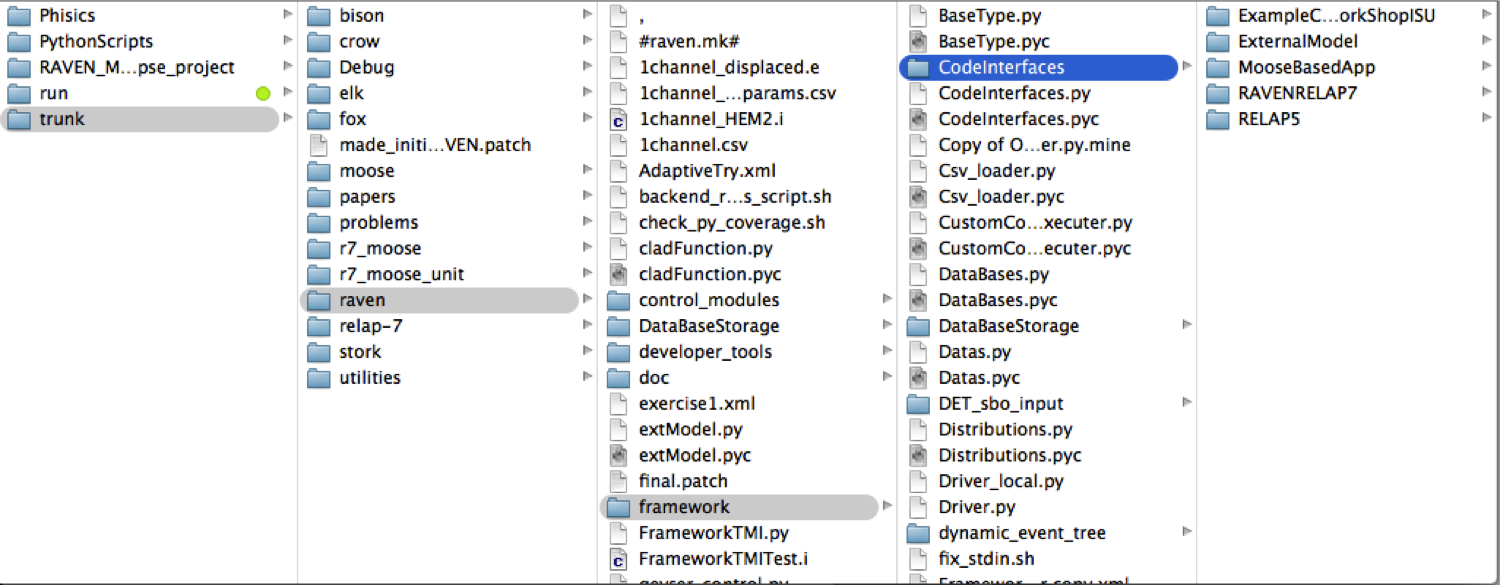
\includegraphics[width=1.0\textwidth]{pics/CodeInterfaceLocation.png}
\caption{Code Interface Location.}
\label{fig:codeinterface}
\end{figure}
The procedure of coupling a new code/application with RAVEN is quite a straightforward process. 
As for all the systems codes currently supported by RAVEN (e.g. RELAP-7, RELAP5-3D, 
BISON, MOOSE, etc.), the coupling is performed through a Python Interface that is in
 charge of interpreting the information coming from RAVEN and translating them in the
  input of the system code under consideration. 
The coupling procedure does not require to modify RAVEN itself. As already mentioned,
 the developer needs to create a new Python interface that is going to be embedded 
 in RAVEN at run-time (no need to introduce  hard-coded coupling statements). 
 This interface needs to be placed in a folder (whatever name) located in (see figure~\ref{fig:codeinterface}):
\begin{lstlisting}[language=bash]
 path_to_raven_distribution/raven/framework/CodeInterfaces/
\end{lstlisting}
At the initialization stage, RAVEN imports all the Interfaces that are contained in the directory above and performs some preliminary cross-checks.
In the following sub-sections, a step-by-step procedure is reported.
\subsection{Pre-requisites.} 
\label{subsec:prerequisites}
In order to couple a newer application to the RAVEN code, some pre-requisites need to be satisfied.
%%% INPUT %%%
\newline
\\\textbf{\textit{\underline{Input}}}
\newline
\\ The first pre-requisite is the knowledge of the input 
syntax of the application the developer wants to couple. Indeed, RAVEN task
 ``ends'' at the Code Interface stage. RAVEN transfers the information needed 
 to perturb the input space into the Code interface and expects that the newly 
 developed Interface is able to perturb the input files based on the information 
 passed through.
\\This means that the developer needs to code a Python-compatible parser of
 the system code input (a module that is able to read and modify the input of 
 the code that needs to be coupled).
\\ For example, let's suppose the input syntax of the code the developer needs 
to couple is as follows:
\begin{lstlisting}[language=python]
  kewword1 =  aValue1
  kewword2 =  aValue2
  kewword3 =  aValue3
  kewword4 =  aValue4
\end{lstlisting} 
The Python input parser would be:
\begin{lstlisting}[language=python]
class simpleInputParser():
  def __init__(self,filename):
    # 
    # @ In, string, filename, input file name (with path)
    #
    self.keywordDictionary = {}
    # open the file
    fileobject = open(filename)
    # store all the lines into a list
    lines = fileobject.readlines()
    # parse the list to construct 
    # self.keywordDictionary dictionary
    for line in lines:
      # split the line with respect
      # to the symbol "=" and store the
      # outcomes into the dictionary
      # listSplitted[0] is the keword
      # listSplitted[1] is the value
      listSplitted = line.split("=")
      keyword = listSplitted[0]
      value   = listSplitted[1]
      self.keywordDictionary[keyword] = value
    # close the file
    fileobject.close()
   
  def modifyInternalDictionary(self,inDictionary):
      # 
      # @ In, dictionary {keyword:value}, 
      # inDictionary, dictionary containing
      # the keywords to perturb 
      #

    # we just parse the dictionary and replace the
    # matching keywords
    for keyword,newvalue in inDictionary.items():
      self.keywordDictionary[keyword] = newvalue

  def writeNewInput(self,filename):
    #
    # @ In, string, filename, newer input file name (with path)
    #

    # open the file
    fileobject = open(filename)
    # write line by line
    for keyword,newvalue in self.keywordDictionary.items():
      fileobject.write(keyword + ``='' + str(newvalue) + ``\n'')
    # close the file
    fileobject.close()
\end{lstlisting} 
%%% OUTPUT %%%
\textbf{\textit{\underline{Output}}}
\newline
\\RAVEN is able to handle Comma Separated Value (CSV) files (as outputs 
of the system code). In order make RAVEN able to retrieve the information
 from the newly coupled code, these files need to be  either generated by the 
 system code itself or the developer needs to code a Python-compatible 
module to convert the whatever code output format to a CSV one. 
This module can be  directly called in the new code interface (see following section).
\\ Let's suppose that the output format of the code (the same of the previous 
input parser example) is as follows:
\begin{lstlisting}[language=python]
  result1 = aValue1
  result2 = aValue2
  result3 = aValue3
\end{lstlisting} 
The Python output converter would be as simple as:
\begin{lstlisting}[language=python]
def convertOutputFileToCSV(outputfile):
    keywordDictionary = {}
    # open the original file
    fileobject = open(outputfile)
    outputCSVfile = open (outputfile + '.csv')
    # store all the lines into a list
    lines = fileobject.readlines()
    # parse the list to construct 
    # self.keywordDictionary dictionary
    for line in lines:
      # split the line with respect
      # to the symbol "=" and store the
      # outcomes into the dictionary
      # listSplitted[0] is the keword
      # listSplitted[1] is the value
      listSplitted = line.split("=")
      keyword = listSplitted[0]
      value   = listSplitted[1]
      keywordDictionary[keyword] = value
    outputCSVfile.write(','.join(keywordDictionary.keys()))
    outputCSVfile.write(','.join(keywordDictionary.values()))
    outputCSVfile.close()
\end{lstlisting} 
And the output CSV becomes:
\begin{lstlisting}[language=python]
  result1, result2, result3
  aValue1, aValue2, aValue3 
\end{lstlisting} 
%%%%%%%
\subsection{Code Interface Creation} 
\label{subsec:codeinterfacecreation}
As already mentioned, RAVEN imports all the ``Code Interfaces'' at run-time, 
without actually knowing the syntax of the driven codes. In order to make RAVEN
able to drive a newer software, the developer needs to code a Python module 
that will contain few methods (with strict syntax) that are called by RAVEN during the simulation.
\\ When loading a ``Code Interface'', RAVEN expects to find, in the class representing the code,
 the following functions:
\begin{lstlisting}[language=python]
from CodeInterfaceBaseClass import CodeInterfaceBase
class NewCode(CodeInterfaceBase):
  def generateCommand(self, inputFiles, executable, flags = None)
  def createNewInput(self, currentInputFiles, oriInputFiles,
                                samplerType, **Kwargs)                           
  def finalizeCodeOutput(self, command, output, workingDir)
  def getInputExtension(self)
  def checkForOutputFailure(self, output, workingDir)
\end{lstlisting} 
In the following sub-sections all the methods are fully explained, providing examples
 (referring to the simple code used as example for the previous sections)
\subsubsection{Method: \textit{def generateCommand(self, inputFiles, executable)}} 
\label{subsubsec:generateCommand}
The \textbf{generateCommand} method is used to retrieve the command 
(in string format) needed to launch the driven Code and the root of the newer output (string).
 In other words, this 
method needs to return a string containing the full command 
that the internal JobHandler is going to use to run the Code this interface refers to. 
Hence, the return data type must be a TUPLE.
\\RAVEN is going to call this function passing in the following arguments:
\begin{itemize}
  \item \textbf{\textit{inputFiles}}, data type = list: List of input files (lenght of the list depends on the 
           number of inputs  have been added in the Step is running this code);
  \item \textbf{\textit{executable}} , data type = string, executable name with absolute 
            path \\(e.g. /home/path\_to\_executable/code.exe);
  \item  \textbf{\textit{flags}} , data type = string, a string containing the flags the 
               user can specify in the input (e.g. under the node $<Code><flags>-u -r</flags></Code>$).
\end{itemize}
For the example referred in the previous section, this method would be implemented as follows:
\newline
\begin{lstlisting}[language=python]
  def generateCommand(self,inputFiles,executable,flags=None):
    found = False
    for index, inputFile in enumerate(inputFiles):
      if inputFile.endswith(self.getInputExtension()):
        found = True
        break
    if not found: raise Exception(``NEWER CODE ERROR ->
                      None of the input files has one of the
                      following extensions ".i", ".inp"!'')
    outputfile = 'out~'+
       os.path.split(inputFiles[index])[1].split('.')[0]
    if flags: precommand = executable + flags
    else    : precommand = executable
    executeCommand = (precommand +
       `` -i '' +os.path.split(inputFiles[index])[1])
    return executeCommand,outputfile
\end{lstlisting} 
\subsubsection{Method: \textit{def createNewInput(self,currentInputFiles,
                                       \\oriInputFiles, samplerType,**Kwargs)}} 
\label{subsubsec:generateCommand}
The \textbf{createNewInput} method is used to generate an input based 
on the information RAVEN passes in. In this function the developer needs to 
call the driven code input parser in order to modify the input file, accordingly with
respect to the variables RAVEN is providing. This method needs to return a list containing 
the path and filenames of the modified input files. \nb RAVEN expects that at least one input 
file of the original list gets modified and re-named.
\\RAVEN is going to call this function passing in the following arguments:
\begin{itemize}
  \item \textbf{\textit{currentInputFiles}}, data type = list: List of current 
              input files (input files from last this method call);
  \item \textbf{\textit{oriInputFiles}} , data type = list, List of the original input files; 
  \item  \textbf{\textit{samplerType}} , data type = string, Sampler type (e.g. MonteCarlo,
               Adaptive, etc.). \nb None if no Sampler has been used;
  \item  \textbf{\textit{Kwargs}} , data type = kwarded dictionary, dictionary of parameters.
               In this dictionary there is another dictionary
               called "SampledVars" where RAVEN stores the 
               variables that got sampled 
               (Kwargs['SampledVars'] => {'var1':10,'var2':40});
\end{itemize}
For the example referred in the previous section, this method would implemented as follows:
\newline
\begin{lstlisting}[language=python]
  def createNewInput(self,currentInputFiles,
        oriInputFiles,samplerType,**Kwargs):
    for index, inputFile in enumerate(inputFiles):
      if inputFile.endswith(self.getInputExtension()):
        break
    parser = simpleInputParser(currentInputFiles[index])
    parser.modifyInternalDictionary(**Kwargs['SampledVars'])
    temp = str(oriInputFiles[index][:])
    newInputFiles = copy.copy(currentInputFiles)
    newInputFiles[index] = os.path.join(os.path.split(temp)[0],
           Kwargs['prefix']+"~"+os.path.split(temp)[1])
    parser.writeNewInput(newInputFiles[index])
    return newInputFiles
\end{lstlisting} 
\subsubsection{Method: \textit{getInputExtension(self, command, output, workingDir)}} 
\label{subsubsec:getInputExtension}
The \textbf{getInputExtension} function is an optional method. If present, it is called 
by RAVEN code at run time.  This function can be considered an utility method, since its
main goal is to return a tuple of strings, where the developer can place all the input extensions
the code interface needs to support (i.e. the extensions of the input(s) the code interface
is going to ``perturb''). If this method is not implemented, the default extensions are  \textbf{(``.i'',' ``.inp'', ``.in'')}.
This function does not accept any input argument.
For the example referred in the previous section, this method would implemented as follows:
\newline
\begin{lstlisting}[language=python]
def getInputExtension(self):
    return (``.i'',``.input'')
 \end{lstlisting} 
\subsubsection{Method: \textit{finalizeCodeOutput(self, command, output, workingDir)}} 
\label{subsubsec:finializeCodeOutput}
The \textbf{finalizeCodeOutput} function is an optional method. If present, it is called 
by RAVEN code at the end of each run. It can be used for those codes, that do not create CSV 
files as output to convert the whatever output format into a CSV. RAVEN checks if a string is returned; 
if so, RAVEN interprets that string as the new output file name (CSV).
\\RAVEN is going to call this function passing in the following arguments:
\begin{itemize}
  \item \textbf{\textit{command}}, data type = string: the command used to run 
                    the just ended job;
  \item \textbf{\textit{output}}, data type = string,the Output name root;
  \item  \textbf{\textit{workingDir}}, data type = string, current working directory.
\end{itemize}
For the example referred in the previous section, this method would implemented as follows:
\newline
\begin{lstlisting}[language=python]
def finalizeCodeOutput(self, command, output, workingDir)
    outfile = os.path.join(workingDir,output+'.o')
    outputobj=convertOutputFileToCSV(outfile)
 \end{lstlisting} 
 
 \subsubsection{Method: \textit{checkForOutputFailure(self, output, workingDir)}} 
\label{subsubsec:checkForOutputFailure}
The \textbf{checkForOutputFailure} function is an optional method. If present, it is called 
by RAVEN code at the end of each run. This method needs to be implemented by the codes that, if a run fails, return a ``returncode'' = 0. 
This can happen in those codes that record the failure of a run (e.g. not converged, etc.) as normal termination (returncode == 0)
This method can be used, for example, to parse the outputfile looking for a special keyword that testifies that a particular job  failed
 (e.g. in RELAP5 would be the keyword "********"). This method MUST return a boolean (True if failed, False otherwise).
\\RAVEN is going to call this function passing in the following arguments:
\begin{itemize}
  \item \textbf{\textit{output}}, data type = string,the Output name root;
  \item  \textbf{\textit{workingDir}}, data type = string, current working directory.
\end{itemize}
For the example referred in the previous section, this method would implemented as follows:
\newline
\begin{lstlisting}[language=python]
def checkForOutputFailure(self, command, output, workingDir)
    from  __builtin__ import any 
    errorWord = "ERROR"
    return any(errorWord in x for x in 
      open(os.path.join(workingDir,output+'.o'),"r").readlines())
 \end{lstlisting} 
 


